\section{Конструкторский раздел}

\subsection{Модели базы данных}

\begin{frame}

\begin{itemize}
    \item Users --- таблица с данными о пользователях.
    \item Projects --- таблица с основными данными о проектах.
    \item ProjectSchemas --- таблица с данными о схемах проектов.
    \item ProjectGrants --- таблица с данными о возможности пользователей размечать данные проектов.
    \item Tasks --- таблица с данными о элементах выборки
    \item LabeledTasks --- таблица с данными о метках
    \item Sessions --- таблица с данными о сессиях пользователей
\end{itemize}


\end{frame}

\subsection{Схема базы данных}

\begin{frame}
    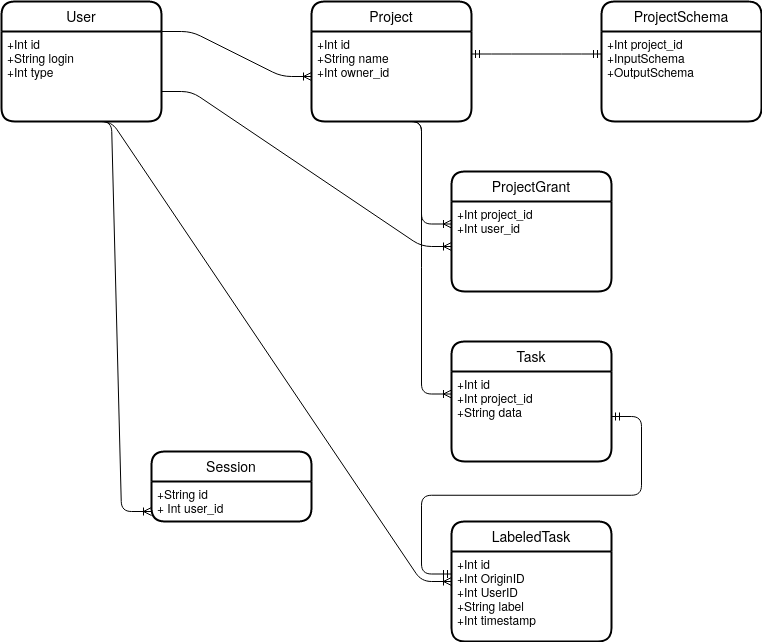
\includegraphics[width=0.8\textwidth]{./dbschema.png}
\end{frame}


\subsection{Классы компоненты доступа к данным}
\begin{frame}
    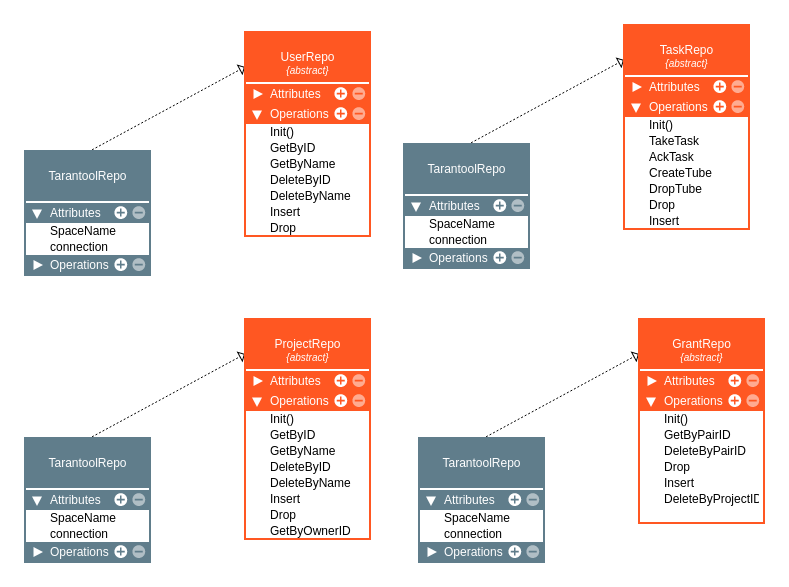
\includegraphics[width=0.9\textwidth]{./dataaccess.png}
\end{frame}

\subsection{Классы компоненты бизнес-логики}

\begin{frame}
    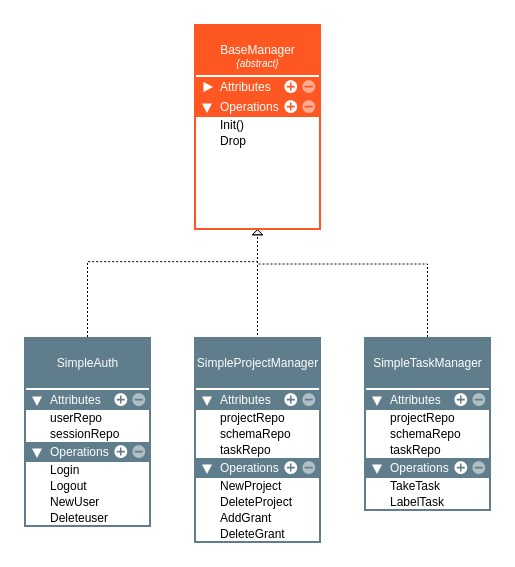
\includegraphics[width=0.8\textwidth]{./business.png}
\end{frame}

\subsection{Классы схем данных}

\begin{frame}
    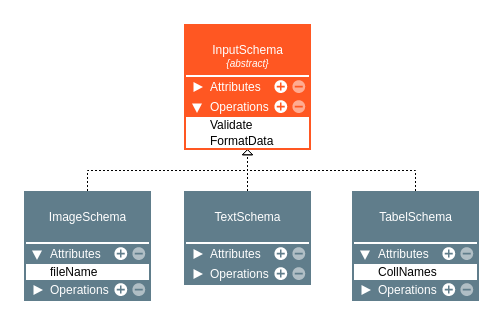
\includegraphics[width=0.9\textwidth]{./inputschema.png}
\end{frame}

%\subsection{Диаграмма классов представлений}

%\begin{frame}
%    \includegraphics[width=1\textwidth]{./views2.png}
%\end{frame}
